\documentclass[journal]{IEEEtai}

\usepackage[colorlinks,urlcolor=blue,linkcolor=blue,citecolor=blue]{hyperref}

\usepackage{color,array}
\usepackage{pst-3dplot}
\usepackage{graphicx}
\usepackage{bm}
\usepackage{listings}
\usepackage[justification=centering]{caption}
\usepackage{amsmath}
\usepackage{subcaption}
\usepackage{pgfplots}
\pgfplotsset{compat=newest}


%% \jvol{XX}
%% \jnum{XX}
%% \paper{1234567}
%% \pubyear{2020}
%% \publisheddate{xxxx 00, 0000}
%% \currentdate{xxxx 00, 0000}
%% \doiinfo{TQE.2020.Doi Number}

\newtheorem{theorem}{Theorem}
\newtheorem{lemma}{Lemma}
\setcounter{page}{1}
%% \setcounter{secnumdepth}{0}


\begin{document}


\title{Pathway for Energy Based Models} 


\author{Germán González, gonzalezv.germanh@javeriana.edu.co }


\markboth{ Artificial Intelligence, Universidad Javeriana de Colombia, November 2022}
{Germán González : Energy Based Models}

\maketitle
\captionsetup{font=footnotesize,justification=justified}
\begin{abstract}

\end{abstract}
  
 

\begin{IEEEkeywords}
Gabor filters, Modern Hopfield networks, Convolutional Networks, Associative memory.
\end{IEEEkeywords}


\section{Introduction}
One of the main field of research on AI is becoming the analysuis of Energy Based Models. The article "Attention is All You need" has had a tremendous impact in the advance of artificial intelligence. And  the recent "Hopfield Networks is all you need" has shown that the Energy based models is the way to go in terms of modeling. However, the theory that backs them is not clearly understood, eventhough it promises that there is a resemblance between biology and the models that path is difficult to follow up. In order to cover that gap, this article will approach the models from two main stating points: The linear associative models that back the idea of attention mchanisms and energy models starting from the Ising model. In general article will be structured in the following mode:

\begin{enumerate}
  \item \textbf{Previous work}
  \item \textbf{Associative memories}
  \item \textbf{Differential equations, eigenvalues and eigenvectors}
  \item \textbf{Hamiltonian dynamics}
  \item \textbf{Clasical Hopfield network}
  \item \textbf{Modern Hopfield networks}
  
\end{enumerate}

\section{Previous work}
Energy Based Models can be traced back to the clasical Hopfield networks \cite{Hopfield}. 
The article "Hopfield Networks is all you need"  treats an extension of the classical Hopfield networks allowing the storage of exponentially more records that the ones possible in the classical networks. This has led then to focus on the investigation about energy Based Models as depicted in the recent article by Yann LeCun "A path towards autonomous machile learning" \cite{Path}. 

\section{Associative memories}
It is know that the human memory is associative. That is to say, that the human needs to have a cue of information in order to correalte the rest of a recall. The memory is built up  day after day from a colection of information that somehow gets store in the brain (Hebbian Learning). \\


The intuition of association can be explained as in the following figure. A person might have two recalls that are totally uncorrelated. However, the presence of a third recall might bring a link between the two so that getting to remeber one induces the recall of another one. When the process only leads to getting to get the full recovery of the recall, then we just have a completition process while, in the case of linking to another recall might lead to and induction process.\\ However, in this article, the process of induction will not be analyzed.

To understand the process of associative learning it is necessary to go back to the theory of eigenvalues and eigenvectors. The reason why the theory was develped was help resolving systems of diferential equations of first order. 
\begin{equation}\label{equ1}
\dot{x}=\textbf{A}x
\end{equation}

The objective is to transform the system in a system where the \textbf{A} matrix is replaced with a diagonal \textbf{D} matris that is easy to solved.

\begin{equation}\label{equ2}
\dot{z}=\textbf{D}z
\end{equation}


The eingenvector and eigenvalues comes from a change of coordinates as follows:
\begin{equation}\label{equ3}
x=Tz
\end{equation}
Deriving it:
\begin{equation}\label{equ4}
\dot{x}=\textbf{T}\dot{z}
\end{equation}
From equation \ref{equ1}:
\begin{equation}\label{equ5}
\textbf{T}\dot{z}=\textbf{A}\textbf{T}\dot{z}
\end{equation}
\begin{equation}\label{equ6}
\textbf{T'}\textbf{T}\dot{z}=\textbf{T'}\textbf{A}\textbf{T}\dot{z}
\end{equation}
\begin{equation}\label{equ7}
\dot{z}=\textbf{T'}\textbf{A}\textbf{T}\dot{z}
\end{equation}
In this last equation \textbf{T'}\textbf{A}\textbf{T} can by identified as:
\begin{equation}\label{equ8}
\textbf{T'}\textbf{A}\textbf{T}=\mathbf{\Lambda}
\end{equation}
So, in the equation \ref{equ2} we can identify $\Lambda$ as the \textbf{D} matrix which is a diagonal matrix of the eigenvalues of \textbf{A}.\\
For example, consider the following system of non linear differental equations:
\begin{equation}\label{equ9}
\begin{array} {rcr}
\dot{x}& =-0.4x + 0.02xy\\
\dot{y}&= 0.8y - 0.01y^2x - 0.1xy 
\end{array}
\end{equation}
The equation has a complex eigenvalue 0.8-2,8i near the point (6,20) when the Jacobian of the equation \ref{equ9} is evaluated in that point,  meaning that any starting point in the right quadrant will converge to it. 
\begin{figure}
\centering
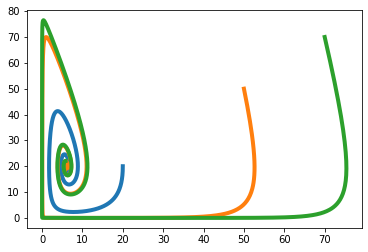
\includegraphics[width=\linewidth]{SINK.png}
\caption{Phase diagram of the system non linear differential equations \ref{equ9}. The lines blue, orange and green indicate the trayectories of three starting points converging to the sink point 6,20. This can be seen as an associative memory that once given certain inofrmation is able to get to the stored memory by itself. }
 \label{fig:SINK}
\end{figure}
  
Now that is clear that a system of differetial equiation with complex eigenvalues can represent memory let´s analyze the propertis of a matrix to store them. Consider a set of orthogonal vectors $v^{(j)}$, j = 1,2,3,..n where $v^{(j)T}v^{j}=0$
\begin{equation}\label{equ10}
\textbf{W}=\sum_{j=1}^{r} v^{(j)T}v^{j}=\textbf{V}\textbf{V}^T
\end{equation}
And getting back to a linear system as in \cite{gBSB}:

\begin{equation}\label{equ11}
\textbf{y}=\textbf{W}\textbf{x}
\end{equation}
Where $\textbf{x}$=$\textbf{v}^{k}$, then:
\begin{equation}\label{equ12}
\textbf{y}=\textbf{W}\textbf{v}^{(k)}=\sum_{j=1}^{r} v^{(j)T}v^{j}v^{(k)}
\end{equation}
\begin{equation}\label{equ13}
=v^{(k)T}v^{k}v^{(k)}=cv^{(k)}
\end{equation}
So, the output can be taken as a linear combination of the inputs. If the vector $\textbf{v}^{(k)}=\textbf{v}^{(k1)}+\textbf{v}^{(k2)} $, where $\textbf{v}^{(k1)} and \textbf{v}^{(k2)}$ are orthogonal, presenting partial information in the form of $\textbf{v}^{(k1)}$:
\begin{equation}\label{equ14}
\textbf{y}=\textbf{W}\textbf{v}^{(k1)}
\end{equation}
Produces:
\begin{equation}\label{equ15}
\textbf{W}=\sum_{j=1}^{r} v^{(j)T}v^{j}v^{k1}
\end{equation}
\begin{equation}\label{equ16}
= v^{k}v^{(k)T}v^{k1}
\end{equation}
\begin{equation}\label{equ17}
= (v^{k1}+v^{(k2)})(v^{k1}+v^{(k2)})^Tv^{k1} 
\end{equation}
\begin{equation}\label{equ18}
= (v^{k1}+v^{(k2)})v^{(k1)T})^Tv^{k1} 
\end{equation}
\begin{equation}\label{equ19}
= dv^{k1} 
\end{equation}
The equation \eqref{equ19} is what is called a Content addressable memory.
\section{Attention mechanism}

As mentioned at the begining in \cite{Attention}, the attention mechanismo is derived from:

\begin{equation}\label{equ20}
Attention(Q,K,V) = softmax(\frac{QK^{T}}{\sqrt{d_{k}}})V 
\end{equation}
The equation above means that attention is a linear combination as expressed down below:
\begin{equation}\label{equ21}
\textbf{y} = \sum_{j=1}^{N}\alpha_{i}\textbf{v}_{i}
\end{equation}
Where:
\begin{equation}\label{equ22}
\sum_{j=1}^{N}\alpha_{i}=1
\end{equation}
To avoid scaling up the input.
In equation \ref{equ20} we see that there is  a factor $\sqrt(d)$ that is similar to the factor d in equation \ref{equ19}, so it leads to consider also that the product $\textbf{QK}^T$ can be replaced by $\textbf{V}^T\textbf{V}$ and finally multiplying  by $\textbf{V}$ and adding over all N we get to an equation simillar to \ref{equ12} where the softmax accounts for the non-orthoganality of the $v^{k}$ vectors.


\section{Softmax interpretation}

The intepretation of the softmax can be deduced from the entropy function \cite{MDF}. Assuming the multiplicity $\text{W}$ of a combinatorial event:

\begin{equation}\label{equ23}
W = \frac{N!}{n1!n2!...n_{t}!•}
\end{equation}

Using the Stirling approximation $x!\approx(x/e)^{x}$:

\begin{equation}\label{equ24}
W = \frac{(N/e)^{N}}{(n1/e)^{n1}...(n_{t}1/e)^{n_{t}}}
\end{equation}
\begin{equation}\label{equ25}
= \frac{(N)^{N}}{(n1)^{n1}...(n_{t}1)^{n_{t}}}=\frac{1}{p^{1}_{n_{1}}...p^{t}_{n_{t}}}
\end{equation}
Then:
\begin{equation}\label{equ26}
ln\, W =- \sum^{t}_{1}n_{i}ln\,p_{i} = \frac{S}{k}
\end{equation}
The equallity \eqref{equ26} is the entrophy divided by the Bolztmann contant. In the mean time wil will no worry about it. What is important it to to find a probablity distribution that obeys that constrains of an energy system and the probabilty sum and also maximizes the entropy. That is to say:
\begin{equation}\label{equ26}
\sum^{t}_{1}p_{i} = 1
\end{equation}
And the average energy: 
\begin{equation}\label{equ27}
\epsilon=\frac{E}{N} = \sum^{t}_{1}\epsilon_{i}p_{i}
\end{equation}
The solution to that is:
\begin{equation}\label{equ28}
p^{*}_{i} = \frac{e^{\beta\epsilon_{i}}}{\sum^{t}_{1}n_{i}e^{\beta\epsilon_{i}}}
\end{equation}
Equation \eqref{equ28} shows that the softmax function is indeed the probability of and event that maximizes the entrophy. In other words is telling you what is the most probable macrostate possible(in terms of thermodynamics) taking certain input.

\section{lagrangian and Hamiltonian dynamics}

In order to study certain Energy based models it is necessary to understand the foundation of classical mechanics. The idea is that knowing the differential equations of a neural networks it is then possible to derive an energy model that can help to model a system.

\subsection{Lagrangian mechanics}

The root of Lagrangian mechanics come from the minimization of the atcion. Assuming that a system is decribed in generalize coordinates. The action is expressed as in equation \eqref{equ30}

\begin{equation}\label{equ30}
S = \int_{x_{1}}^{x_{2}}L(\textbf{q},\dot{\textbf{q}},t)dt
\end{equation}
The value of S is maximized or minimized when the Euler-Lagrange \eqref{equ31} holds:
\begin{equation}\label{equ31}
\frac{\partial L}{\partial q}- \frac{d}{dx}\frac{\partial L}{\partial\dot{q}}=0
\end{equation}

\subsection{Hamiltonian mechanics}

As known from clasical mechanics, the Hamiltonian is the total energy of a system as in equation \eqref{equ32}.

\begin{equation}\label{equ32}
H\,= T\, +\, V
\end{equation}
And the Lagrangian is:
\begin{equation}\label{equ33}
L = T\, -\, V
\end{equation}
The Legendre transformation allows us to move from the Lagrangian to the Hamiltonian as follows:
\begin{equation}\label{equ34}
E = \left ( \sum_{n}^{i=1}\dot{q_{i}}\frac{\partial L}{\partial \dot{q}} \right )-L
\end{equation}

\section{Biological Model}
The article from Hodkin-Huxley describes the dinamic equations of the action potencial \cite{Hodgkin}. The figure \ref{fig:HH} shows the diagram that resembles the model. The equations that govern the model are the folllowing:
\begin{figure}
\centering
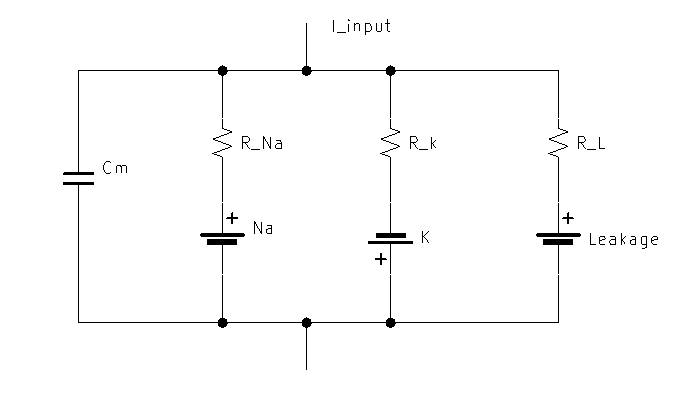
\includegraphics[width=\linewidth]{Hodgkin_Huxley.png}
\caption{The electrical equivalent circuit of the Hogdkin Huxley Model \cite{Huxley}.}
 \label{fig:HH}
\end{figure}
\begin{equation}\label{equ35}
I = C_{m}\frac{dV}{dt}+I_{input}
\end{equation}
The total input current is:
\begin{equation}\label{equ36}
I = I_{NA}+I_{K}+I_{l}
\end{equation}
The Currents as in equations \eqref{equ35} are the Sodium (Na), Potasium (K) and a Leakage current (l). Those current have associated conductances $g_{Na}$, $g_{K}$ and  $g_{l}$.  However, the conductances are non-lineal fuctions as they obey diffusion laws. Therefore:
\begin{equation}\label{equ37}
I = C_{m}\frac{dV}{dt}+\overline{g}_{K}n^{4}(V-V_{K})+\overline{g}_{Na}m^{3}(V-V_{Na})+\overline{g}_{l}(V-V_{l})
\end{equation}
Where:
\begin{equation}\label{equ38}
\frac{dn}{dt}=\alpha_{n}(1-n)-\beta_{n}n
\end{equation}
\begin{equation}\label{equ39}
\frac{dm}{dt}=\alpha_{m}(1-n)-\beta_{m}m,
\end{equation}
\begin{equation}\label{equ40}
\frac{dh}{dt}=\alpha_{h}(1-n)-\beta_{h}h
\end{equation}
In the above equations, the fact that they vary acccording to the voltage, allows the spikes to present transient forms different from the ones present in an electric RC circuit as in the figure \ref{fig:HH2}.

\begin{figure}
\centering
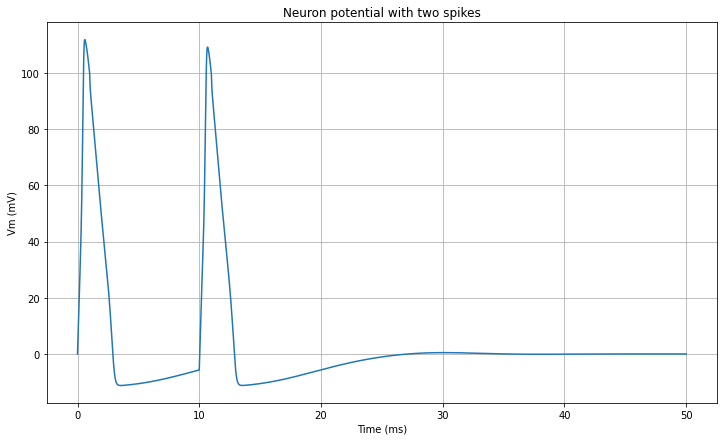
\includegraphics[width=\linewidth]{spikes.png}
\caption{The electrical response of a Hogdkin Huxley Model.}
 \label{fig:HH2}
\end{figure}

Taking into account the equation \eqref{equ37}. The model can be rewritten as:
\begin{equation}\label{equ41}
I=C_{m}\frac{dV}{dt}+ \sum^{N}_{i=1}M_{\mu i} g_{i}
\end{equation}
Reweriting it:
\begin{equation}\label{equ41}
\tau \frac{dV}{dt}= \sum^{N}_{i=1}\xi_{\mu i} g_{i}-I
\end{equation}

\section{Large Asociative Memory Problem}
In the article \cite{Krotov}. Krotov and Hopfield address the problem of creating a plausible energy model. The model is based on RBM\footnote{Boltzmann Machines} and deduce the equations for a feature and hidden layers. The equatiosn are:

And get transformed into Hamiltonian energy models via a Legendre transformation.
  
%%\section{Ising model and Hopfield model}
%%So far we have see how an attention mechanism is the statistical pair of linear associative model, however, it is not yet connected to any natuaral process. To start getting a connection, it is necessary to understand what the ising model is and how it is formulated.\\
%%The Ising model is a model for the ferromagnetic behaviour of certain materials and it is model out from the Hamiltonian of the energy as in equation \ref{equ23}:
%%\begin{equation}\label{equ23}
%%E=-\frac{1}{2}\sum_{i,j=1}^{N}\sigma_{i}T_{ij}\sigma{j}, \: T_{ij}=\sum_{i,j=1}^{K}\xi^{u}_{i}\xi^{u}_{j}
%%\end{equation}
%%The first term in \ref{equ23} is similar to equation \ref{equ12}. theerfore it is necessary to understand the properties of the right side of equation \ref{equ23}.


\begin{thebibliography}{34}
\setcounter{enumiv}{0}

\bibitem{programs} Brain model. (2021, 11 25). {\em Brain Model}. [Notebook]. Available at $https://github.com/ghgv/Brain_model$

\bibitem {Hartline} H. K. Hartline, 'The response of single optic nerve fibers of the vertebrate eye to illumination of the retina', {\em Am J Physiol} vol 121, pp :400–415, 1938

\bibitem{Hubel} D. H. Hubel, T. N. Wiesel,'Receptive fields of single neurones in the cat's striate cortex' {\em J. Physiol},,pp 574-591,1959

\bibitem{MDF} Ken A. Dill, Sarina Bromberg,'Molecular Driving Forces, Statistical Thermodynamics in Biology Chemistry, Physics, and Nanoscience, 2nd ed.' {\em },,pp 574-591,1959

\bibitem{Path} LeCun, Yann, 'A Path Towards Autonomous Machine Intelligence'{\em} , 2022.


%%\bibitem{}J. S. Turner, ``New directions in communications,'' {\em IEEE J. Sel. Areas Commun.}, vol. 13, no. 1, pp. 11--23, Jan. 1995. 

\bibitem{McCulloch} McCulloch, Warren S and Pitts, Walter,'A logical calculus of the ideas immanent in nervous activity' {\em The bulletin of mathematical biophysics.},vol. 5, no. 4, pp. 115-133,1943.

\bibitem{Hodgkin} A. L. Hodgkin and A.F. Huxley,'A quantitative description of membrane current and its application to conduction and excitation in nerve' {\em Physiological Laboratory, University of Cambridge.},1952

%%\bibitem{Minsky} Minsky, Marvin L.,'Computation: Finite and Infinite Machines' {\em Prentice-Hall, Inc.},1967

\bibitem{Hopfield} Hopfield, J J.,'Neural networks and physical systems with emergent collective computational abilities' {\em Proceedings of the National Academy of Sciences },pp 2554-2558, 1982

\bibitem {MHN} Hubert Ramsauer, Bernhard Schaefl,              Johannes Lehner, Philipp Seidl ,Michael Widrich ,               Lukas Gruber, Markus Holzleitner, Milena Pavlovic,               Geir Kjetil Sandve, Victor Greiff, David P. Kreil,
Michael Kopp,Genter Klambauer,Johannes Brandstetter,Sepp Hochreiter, 'Hopfield Networks is all you need',{\em},2021
 
\bibitem {Hebbian} Donald O. Hebb, 'The Organization of Behavior',{\em},1949

\bibitem{Fukushima} Fukushima, K..,'Neocognitron: A self-organizing neural network model for a mechanism of pattern recognition unaffected by shift in position' {\em Biological Cybernetics.},pp. 193-202,1980

%%\bibitem{Llinas} Pellionisz A, Llinás R,'Brain modeling by tensor network theory and computer simulation. The cerebelum processor for predective coordination' {\em Neuroscience.},vol 4, pp 232-348, 1979

%%\bibitem{Manes} Facundo Manes, Mateo Niro,'Usar el Cerebro, conocer nuestra mente para vivir mejor' {\em }, 2014

%%\bibitem{NTM} A. Graves, G. Wayne, I. Danihelka' {\em arXiv:1410.5401.}, 2014

%%\bibitem{Low} F. Effenberger1, C. Hillar,'Discovery of Salient Low-Dimensional Dynamical Structure in Neuronal Population Activity Using Hopfield Networks '{\em} ,2015

%%\bibitem{Ng} A. Coates, H. Lee,Andrew Y Ng,'An Analysis of Single-Layer Networks in Unsupervised Feature Learning'{\em} ,2015

%%\bibitem {Poggio} M. Riesenhuber, T. Poggio,'Hierarchical models of object recognition in cortex' {\em. Nature Neuroscience},1999

\bibitem {gBSB} Oh, Cheolhwan and Stanisław H. Żak. “The Generalized Brain-State-ina-Box ( gBSB ) Neural Network : Model , Analysis , and Applications.” (2005).

\bibitem {Olshausen} B. Olshausen, D. Field,'Emergence of simple cell receptive field properties by learning a sparse code for natural images' {\em Nature}, 1996 

\bibitem {LeCun} Y. LeCun, L. Bottou, Y. Bengio, P. Haffner, ' Gradient-Based Leardning Applied to Document Recognition' {\em Proc. of the IEEE}, 1998


%\bibitem {Hava} Hava T. Siegelmann, 'RECURRENT NEURAL NETWORKS AND FINITE AUTOMATA'{\em Computational Intelligence}, vol 12, No 14, 1996

%%\bibitem{mito} R. Llínas, 'El Cerebro y el mito del yo: el papel de las neuronas en el pensamiento y el comportamiento humanos',{\em El Peregrino Ediciones}, 2017	


\bibitem{Linnainmaa} Seppo Linnainmaa, 'Taylor expansion of the accumulated rounding error'BIT ,{\em  Numerical Mathematics}, vol 16, pages 146–160, 1976

\bibitem {Schiller} Peter H. Schiller, 'Parallel information processing channels created in the retina',{\em Proceedings of the National Academy of Sciences }, 2010

%%\bibitem{Krotov} D. Krotov, J.J. Hopfield, 'Unsupervised learning by competing hidden units', {\em Proceedings of the National Academy of Sciences}, 2019
\bibitem{Krotov} D. Krotov, J.J. Hopfield, 'LARGE ASSOCIATIVE MEMORY PROBLEM IN NEUROBIOLOGY AND MACHINE LEARNING', {\em  ICLR 2021}, 2021


\bibitem {Madathati} N. V. Medathati,H. Neumannb, G.S.Masson,P. Kornprobst, 'Bio-inspired computer vision: Towards a synergistic approach of artificial and biological vision', {\em Elsevier},2016 

\bibitem {Rojas} R. Rojas, 'Neural Network: A Systematic Introduction', {\em Springer},1996

\bibitem {CCP} A.L. Yuille, Anand Rangarajan, 'The Concave-Convex Procedure',{\em Neural Comput},2003

%%\bibitem {Gabor_formula}'$http://vision.psych.umn.edu/users/kersten/kersten-lab/courses/Psy5036W2017/Lectures/17_PythonForVision/Demos/html/2b.Gabor.html$'


%%\bibitem {cortices} '$https://procesamientodelainformacionvisual.files.wordpress.com/2014/04/areas-de-la-corteza-visual.jpg$'

%%\bibitem{Gabor} '$http://vision.psych.umn.edu/users/kersten/kersten-lab/courses/Psy5036W2017/Lectures/17_PythonForVision/Demos/html/2b.Gabor.html$'

\bibitem{Gaborb} '$http://vision.psych.umn.edu/users/kersten/kersten-lab/courses/Psy5036W2017/Lectures/17_PythonForVision-/Demos/html/2b.Gabor.html$'

\bibitem{mit} M. Fee, '$https://Introduction-to-neural-computation-spring-2018/lecture-notes/MIT9_40S18_Lec02.pdf$' 

\bibitem {homer} Johannes Brandstetter, '$https://ml-jku.github.io/hopfield-layers/$'.

\bibitem {Attention}	Attention is all you need,
A. Vaswani, N. Shazeer, N. Parmar, J. Uszkoreit, L. Jones, A. Gomez,  Kaiser, and I. Polosukhin.{\em Advances in Neural Information Processing Systems} , page 5998--6008. 2017

\end{thebibliography}
\
\end{document}